s\chapter{Additions}
\label{chap:additions}


To better handle the parametrized automaton We need to introduce the following definitions.

\section{Tokens and parameters}

\begin{dfn}
	\label{token}
	A (not timed and not parametrized) token is a state.
\end{dfn}

At this point, it this definition seems to be pointless, however it'll help the reader understand the complexity of the parametrized case.
The meaning of the token: It is the only active state of a Deterministic Finite Automaton or one of the multiple active states of a Nondeterministic Finite Automaton.

\begin{dfn}
	\label{timed_token}
	A timed token is tuple $\langle Q, T\rangle$, where
	\begin{itemize}
		\item Q is a state,
		\item and T is a set of currently active timers.
	\end{itemize} 
\end{dfn}

The semantics of each timed token: They contain one of the active states with the currently active clocks which can effect it.

\begin{dfn}
	\label{timed_parametrized_token}
	A timed parametrized token is a tuple $\langle Q, T, P \rangle$, where
	\begin{itemize}
		\item Q is a state,
		\item T is a set of the currently active timers
		\item and P is a Parameter Binding Relation.
	\end{itemize}
\end{dfn}
 
The semantics of each timed parametric token: They contain one of the active states with the currently active clocks, and a Parameter Binding Relation which holds the currently bound parameters.

\todo{Definition for the fixed parameter binding, for the parameters, and stuff like that.}

\begin{dfn}
	\label{parameter_binding_relation}
	\mytodo{Refine this}
	A Parameter Binding Relation $P$, $P_1$, $P_2$ and a fixed parameter binding $F$ has the following operations:
	\begin{itemize}
		\item $P_1 \cup P_2 = P$, e.g. two relations has a union,
		\item $P_1 \setminus F = P$ e.g. two relations has an intersection \mytodo{what?},
		\item Can be checked if it contains anything,
		\item And add every possible parameter value with $\forall$.
	\end{itemize}
\end{dfn}

The Parameter Binding Relation represents the information of the parameters.
The following example will clear up what is the exact purpose of this relation.


\begin{figure}[h]
	\centering
	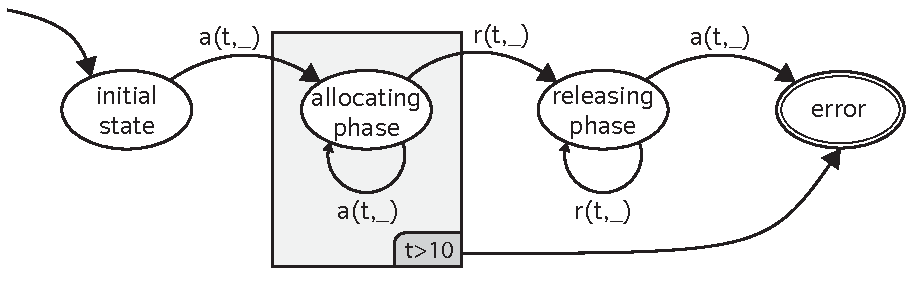
\includegraphics[width=0.7\linewidth]{figures/chapter_4/allocating_timed_parametric}
	\caption{Parametric timed region event automaton of the two phase locking example \redraw}
	\label{fig:cep:ptrea2}
\end{figure}

On \cref{fig:cep:ptrea2} you can see two states called $s_1$ and $s_2$, and one transition with the label $A(t,\mathunderscore)$. When event $A$ occurs, with the parameters of $(1,2)$ the following happens:
\begin{enumerate}
	\item First we create a fixed parameter binding from the event. In this example: $\#\{A \rightarrow 1; B \rightarrow 2\}$,
	\item \label{example_step_2} Then we intersect all of the Parameter Binding Relations on state $s_1$,
	\item And add the result of the previous step % \cref{example_step_2}
	 to $s_2$.
\end{enumerate}
  


\begin{dfn}
	A timed and parametrized token is a tuple $\langle Q,T,P \rangle$, where 
	\begin{itemize}
		\item $Q$ and $T$ are the same as in \cref{timed_token}, and 
		\item $P$ is a Parameter Binding Relation
	\end{itemize}
\end{dfn}

\begin{dfn}
	A set of bound and unbound parameters conforms to an other one when the following applies $\forall$ variables
	\begin{itemize}
		\item Both of them are concrete parameters, and their values are equal.
		\item LHS is a concrete parameter while RHS is an unbound parameter, but LHS's value is not excluded from RHS
		\item Both of them are unbound, and the excluded values of LHS are $\subseteq$ RHS
	\end{itemize}
\end{dfn}
	
\subsection{Possible Data Structures for Parameter Binding Relations}

There are many ways to implement these relations. Three of these have been implemented.

\subsubsection{Decision List}

A decision list is a list of data, where each cell contains either a concrete value or the symbol $\ast$ which stands
for ``anything''. To find out if a values in the relation the rows must be read in order, and find the first row which conforms the values you are searching for \todo{algorithm} \dots and return the containment.
An example of a decision list is shown on \cref{tab:cep:decision_list}

\begin{table}
	\centering
	\caption{An example of a Decision List}		
	\label{tab:cep:decision_list}
	\begin{tabular}{cccc}
		\toprule
		\# & containment & $A$ & $B$ \\
		\midrule
		1 & $+$ & $2$ & $\ast$\\
		2 & $+$ & $3$ & $5$ \\
		3 & $-$ & $\ast$ & $\ast$ \\
		\bottomrule
	\end{tabular}
\end{table}

\subsubsection{Disjunctive Decision Set} \todo{rename}

An event -- in a more formal way -- is a conjunction of a logical statement. When we think of $\mathit{Allocate}(1,2)$ we actually mean that we have an event called $\mathit{Allocate}$ where $\mathit{Task} = 1 $ $\with$ $\mathit{Resource} = 2$.
With this mindset we can assume that a Parameter Binding Relation is actually only a disjunction of such statements.
So when we think of a ``Relation with parameters $\mathit{A}$ and $\mathit{B}$ which contains every pair of numbers
which are odd'' \todo{finish this and refactor}

An example is shown on \cref{tab:cep:dds}.

\begin{table}
	\centering
	\caption{An example of a Disjunctive Decision Set}		
	\label{tab:cep:dds}
	\begin{tabular}{cccc}
		\toprule
		\# & containment & $A$ & $B$ \\
		\midrule
		1 & $+$ & $2$ & $\ast\setminus\{1,2\}$ \\
		2 & $+$ & $3$ & $5$ \\
		3 & $-$ & $\ast$ & $\ast$ \\
		\bottomrule
	\end{tabular}
\end{table}


\subsubsection{MDDe}

MDDe is a Multiple-value Decision Diagram with else branches. We could use simple MDD's with intervals, but in many cases the parameters do not have a supremum and infimum and they are not in a sequence.




